\documentclass[12pt]{article}
\usepackage{graphicx}
\usepackage{enumitem}
\usepackage{amsmath}
\usepackage{gvv-book}
\usepackage{gvv}

\title{\textbf{4.5.7}}
\author{\textbf{Aditya Mishra-EE25BTECH11005}}
\date{September 30, 2025}

\begin{document}

\maketitle

\section*{Question}

The equation of a line, which is parallel to $2\hat{i} + \hat{j} + 3\hat{k}$ and passes through the point $(5, -2, 4)$ is
\[
\frac{x - 5}{2} = \frac{y + 2}{-1} = \frac{z - 4}{3}.
\]


\section*{Solution}

Let the point $\vec{h}$ and direction vector $\vec{m}$ be  

\[
\vec{h} = \myvec{5 \\ -2 \\ 4}, \quad 
\vec{m} = \myvec{2 \\ 1 \\ 3}.
\]

The vector equation of the line is given by
\[
\vec{x} = \vec{h} + \lambda \vec{m}, \quad \lambda \in \mathbb{R}.
\]

Expanding,  
\begin{align}
\vec{x} &= \myvec{5 \\ -2 \\ 4} + \lambda \myvec{2 \\ 1 \\ 3} \\[2mm]
           &= \myvec{5 + 2\lambda \\ -2 + \lambda \\ 4 + 3 \lambda}.
\end{align}

Hence the parametric equations of the line are  
\begin{align}
x &= 5 + 2\lambda, \\
y &= -2 + \lambda, \\
z &= 4 + 3\lambda, \quad \lambda \in \mathbb{R}.
\end{align}

Therefore, the symmetric form of the line is
\[
\boxed{\frac{x - 5}{2} = \frac{y + 2}{1} = \frac{z - 4}{3}}.
\]
Which is different from the equation in the question:
\[
\frac{x - 5}{2} = \frac{y + 2}{-1} = \frac{z - 4}{3}
\]

Hence, the statement:

The equation of a line, which is parallel to $2\hat{i} + \hat{j} + 3\hat{k}$ and passes through the point $(5, -2, 4)$ is $\frac{x - 5}{2} = \frac{y + 2}{-1} = \frac{z - 4}{3}$ is False.
\section*{Plot}
\begin{figure}[H]\centering
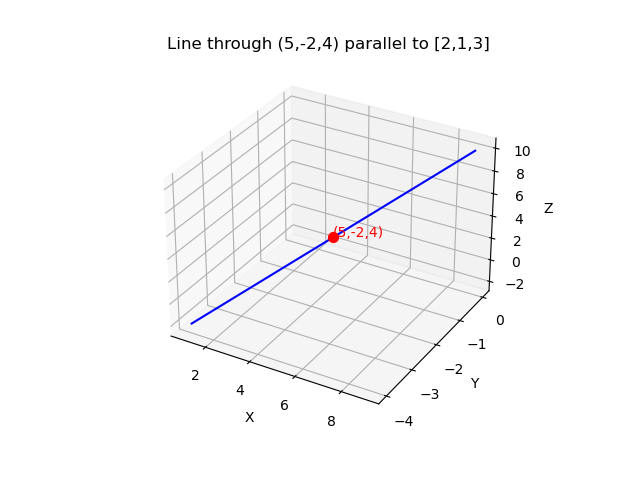
\includegraphics[width=1\columnwidth]{Figs/Figure_1.png}
\caption{3D plot of the line}
\label{fig:plt}
\end{figure}
\end{document}

